\documentclass[12pt]{article}
\usepackage{soul}
\usepackage{tikz}
\usepackage{amsmath}
\usepackage{amsthm}
\usepackage{amssymb}
\usepackage{lipsum}
\usepackage{float}
\usepackage{titlesec}

\usepackage[strict]{changepage} 
\usepackage{framed} 

\usepackage{enumerate}
\usepackage{subfigure}
\usepackage{geometry}
\usepackage{graphicx}
\usepackage{booktabs}
\usepackage{makecell}
\usepackage{xeCJK}
\usepackage{tcolorbox}
\usepackage[dvipsnames]{xcolor}
\setcounter{secnumdepth}{4}
\geometry{a4paper,scale=0.8}
\linespread{1}

\usepackage{pdfpages}
\renewcommand{\baselinestretch}{1.4}

\definecolor{formalshade}{rgb}{0.95,0.95,1} % 文本框颜色

\newenvironment{formal}{%
\def\FrameCommand{%
\hspace{1pt}%
{\color{Blue}\vrule width 2pt}%
{\color{formalshade}\vrule width 4pt}%
\colorbox{formalshade}%
}%
\MakeFramed{\advance\hsize-\width\FrameRestore}%
\noindent\hspace{-4.55pt}% 
\begin{adjustwidth}{}{7pt}%
\vspace{2pt}\vspace{2pt}%
}
{%
\vspace{2pt}\end{adjustwidth}\endMakeFramed%
}

\newcounter{mytheoremcounter}
\newcounter{mydefinitioncounter}
\newcounter{mylemmacounter}
%theorem
\newtcolorbox{mytheorem}[1][]{
    colback=blue!5!white,      
    colframe=Blue,    
    fonttitle=\bfseries,       
       title=Theorem~\refstepcounter{mytheoremcounter}\themytheoremcounter,  
    label=#1                 
}
%definition
\newtcolorbox{mydefinition}[1][]{
    colback=SpringGreen!5!white,     
    colframe=SpringGreen!88!black,     
    fonttitle=\bfseries,       
       title=Definition~\refstepcounter{mydefinitioncounter}\themydefinitioncounter,  
    label=#1                    
}

\newtcolorbox{mylemma}[1][]{
    colback=blue!5!white,     
    colframe=Blue,  
    fonttitle=\bfseries,       
       title=Lemma~\refstepcounter{mylemmacounter}\themytheoremcounter, 
    label=#1                   
}

\titleformat{\section}
  {\large\bfseries}
  {\thesection}    
  {1em}           
  {}               

\newtheorem{theorem}{Theorem}[section]
\newtheorem{definition}{Definition}[section]
\newtheorem{corollary}{Corollary}[theorem]
\newtheorem{lemma}[theorem]{Lemma}

\begin{document}
\begin{center}
\begin{large}
\textbf{Approximation by Superpositions of a Sigmoidal Function}\\
\end{large}
Paper Handout by Zixin Yu
\end{center}

In 1989, Cybenko published a paper titled Approximation by Superpositions of a Sigmoidal Function. In this paper, Cybenko demonstrated that a feedforward neural network with a single hidden layer can approximate any continuous function defined on a compact set. This result later became known as the \textbf{Universal Approximation Theorem}. In this article, I will attempt to outline the entire proof process, clarify some of the points of confusion I encountered during my reading, and provide more in-depth mathematical explanations of the details that Cybenko skipped over. The following content will involve numerous concepts from measure theory and functional analysis, but they are not too difficult. I believe that even without a solid foundation, one can still grasp the essence of the proof.

\section{Problem Description}

\begin{figure}[H]
    \centering
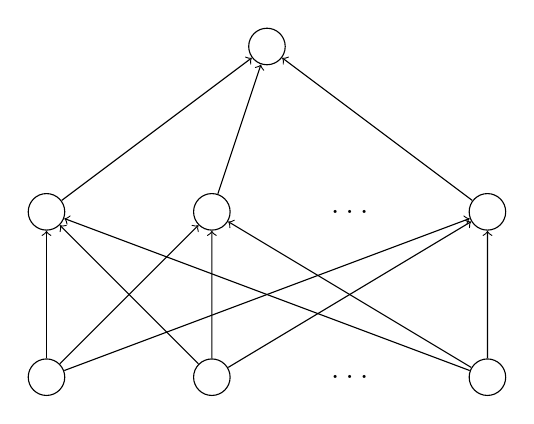
\begin{tikzpicture}[scale=1.4, every node/.style={scale=1.4}]

    \node[circle, draw] (input1) at (0, 0) {};
    \node[circle, draw] (input2) at (1.5, 0) {};
    \node[circle, draw] (input3) at (4, 0) {};
    
    \node[circle, draw] (hidden1) at (0, 1.5) {};
    \node[circle, draw] (hidden2) at (1.5, 1.5) {};
    \node[circle, draw] (hidden3) at (4, 1.5) {};
    \node[circle, draw] (output1) at (2, 3) {};
    
    \node at (2.75, 0) {\scriptsize \(\dots\)};
    \node at (2.75,1.50) {\scriptsize \(\dots\)};
    
    \draw[->] (input1) -- (hidden1);
    \draw[->] (input1) -- (hidden2);
    \draw[->] (input1) -- (hidden3);
    
    \draw[->] (input2) -- (hidden1);
    \draw[->] (input2) -- (hidden2);
    \draw[->] (input2) -- (hidden3);
    
    \draw[->] (input3) -- (hidden1);
    \draw[->] (input3) -- (hidden2);
    \draw[->] (input3) -- (hidden3);
    
    \draw[->] (hidden1) -- (output1);
    \draw[->] (hidden2) -- (output1);
    \draw[->] (hidden3) -- (output1);
    
    \end{tikzpicture}
\end{figure}

A feedforward neural network with a single hidden layer typically takes the following form:
\begin{align*}
    \sum_{j=1}^N \alpha_j \sigma (w_j^T x +\theta_j).
\end{align*}

In the structure of the neural network, $w_j$ represents the weight applied to the input $x$, $\alpha_i$ represents the weight of the output from the hidden layer, and $\theta_i$ is the bias of neuron $i$. We refer to $w_j^T x + \theta_j$ as the affine transformation with respect to the neural network input.\\

Let $I_n$ be the $n$-dimensional unit cube $[0,1]^n$, and denote the space of continuous functions on $I_n$ as $C(I_n)$. The space of finite regular Borel measures on $I_n$ is denoted by $M(I_n)$. We use $\left\lVert f\right\rVert$ to represent the supremum norm of $f \in C(I_n)$, where $\left\lVert \cdot\right\rVert$ is often used to denote the maximum value of a function over its domain. The primary goal of the following proof is to determine the conditions under which functions of the form
\begin{align*}
    G(x)= \sum_{j=1}^N \alpha_j \sigma (w_j^T x +\theta_j)
\end{align*}
are dense in $C(I_n)$ with respect to the supremum norm.

\begin{mydefinition}
If for all $y \in \mathbb{R}^n$ and $\theta \in \mathbb{R}$, the integral with respect to the measure $\mu \in M(I_n)$
    \begin{align*}
        \int_{I_n} \sigma(w^Tx+\theta)\mathrm{d}\mu(x)=0,
    \end{align*}
    implies that $\mu = 0$, then $\sigma$ is said to be discriminatory.
\end{mydefinition}
When I read this definition, I encountered some confusion. It can actually be restated in another way: for a non-zero measure $\mu$, there exist $w_j$ and $\theta_j$ such that
\begin{align*}
\int_{I_n}\sigma(w^Tx+\theta)\mathrm{d}\mu(x)\neq 0
\end{align*}
If the above expression equals zero, then $\mu$ must be the zero measure. More intuitively, a discriminatory $\sigma$ is non-destructive in terms of volume, ensuring that no information is lost when processing the shifted and weighted $x$. Therefore, it will not reduce the affine space $w_j^T x + \theta_j$ to a zero-measure set. Now, let’s look at the definition of a sigmoidal function.

\begin{mydefinition}
    A sigmoidal activation function satisfies
    $$\sigma(t) \to 
    \begin{cases} 
    1, & t \to +\infty \\
    0, &  t \to -\infty.
    \end{cases}$$
\end{mydefinition}
There are many functions that satisfy Definition 2 (such as logistic, softmax, etc.), but here we will only discuss the general case. The second part will present some key results, and the third part will apply these results to the structure of neural networks. The original author also discussed other types of activation functions, but due to time constraints, I’ll leave that for later when I have the chance to fill in the gaps.

\section{Main Results}

\begin{mytheorem}
    Let $\sigma$ be any continuous discriminatory function. Then, functions of the form
    \begin{align}
        G(x)=\sum_{j=1}^N \alpha_j \sigma (w_j^T x +\theta_j)
    \end{align}
    finite sums of such functions are dense in $C(I_n)$. In other words, given any $f \in C(I_n)$ and $\epsilon > 0$, there exists a function $G(x)$ of the above form such that\begin{align*}
        |G(x)-f(x)|<\epsilon, \quad x\in I_n.    \end{align*}
\end{mytheorem}

\begin{proof}
    Let $S \subseteq C(I_n)$ be the set of functions formed by $G(x)$ as defined in equation (1). Clearly, $S$ is a linear subspace of $C(I_n)$. To prove that $S$ is dense in $C(I_n)$, we need to show that the closure of $S$ is the entirety of $C(I_n)$. We use $\overline{S}$ to denote the closure of $S$. If we assume $\overline{S} \neq C(I_n)$, then $\overline{S}$ is a proper closed subspace of $C(I_n)$.
\begin{formal}
\textbf{Hahn-Banach Theorem}\\
Let $S \subseteq C(I_n)$ be the set of functions formed by $G(x)$ as defined in equation (1). Clearly, $S$ is a linear subspace of $C(I_n)$. To prove that $S$ is dense in $C(I_n)$, we need to show that the closure of $S$ is the entirety of $C(I_n)$. We use $\overline{S}$ to denote the closure of $S$. If we assume $\overline{S} \neq C(I_n)$, then $\overline{S}$ is a proper closed subspace of $C(I_n)$.
\end{formal}

The Hahn-Banach theorem provides us with a method to extend a bounded linear functional defined on $S$ to a bounded linear functional defined on the entire $C(I_n)$. According to the Hahn-Banach theorem, there exists a bounded linear functional on $C(I_n)$, denoted as $L$, such that
\begin{align*}
    L(S)=L(\overline{S})=0,\quad L\neq 0
\end{align*}

\begin{formal}
\textbf{Riesz Representation Theorem}\\
Let $X$ be a locally compact Hausdorff space, and let $C_c(X)$ be the set of continuous functions with compact support defined on $X$. For each positive linear functional $\Lambda$ on $C_c(X)$, there exists a unique positive and regular Borel measure $\mu$ such that for all $f \in C_c(X)$, the following holds:
$$\Lambda(f) = \int_X f d\mu.$$
The measure $\mu$ is regular, meaning it satisfies the following properties:
\begin{itemize}
    \item For any open set \( U \subset X \),
    $
    \mu(U) = \sup \{ I(f) : f \in C_c(X), f \in [0,1], \text{supp } f \subset U \}.
    $
    \item For any compact set \( K \subset X \),
    $
    \mu(K) = \inf \{ I(f) : f \in C_c(X), f \geq \chi_K \}.
    $
\end{itemize}
\end{formal}
The measure $\mu$ is regular, meaning it satisfies the following properties:
\begin{align*}
    L(h)=\int_{I_n} h(x)\mathrm{d}\mu(x).
\end{align*}
For any $w$ and $\theta$, functions of the form $\sigma(w^T x + \theta)$ are all in $S$, and since $L$ is zero on $S$, we have the following result:
\begin{align*}
    \int_{I_n} \sigma(w^Tx+\theta)\mathrm{d}\mu(x)=0.
\end{align*}
Since $\sigma$ is a discriminatory function, we must have $\mu = 0$. This contradicts the conclusion that $L \neq 0$, because:
\begin{align*}
    \mu=0 \implies \int_{I_n} h(x)\mathrm{d}\mu(x)=0,\quad h\in C(I_n)
\end{align*}
Therefore, $S$ is dense in $C(I_n)$. Q.E.D.

\end{proof}

\begin{mylemma}
    Any continuous sigmoidal function is discriminatory.
\end{mylemma}
Recalling the definition of a discriminatory function, we need to examine the case where $\int_{I_n} \sigma(w^T x + \theta) \, \mathrm{d}\mu(x) = 0$. This is an integral over a measure space, which can be approached by constructing a sequence of non-negative simple functions that monotonically increase and approximate the original function, thereby simplifying the expression.

\begin{proof}
    Note that for any $x$, $w$, $\theta$, and $\varphi$, we have the following:
\begin{align*}
    \sigma(\lambda (w^T x + \theta) + \varphi) \rightarrow 
\begin{cases}
1, &  \quad w^T x + \theta > 0 \quad \text{as} \quad \lambda \to +\infty, \\
0, &  \quad w^T x + \theta < 0 \quad \text{as} \quad \lambda \to +\infty, \\
\sigma(\varphi), & \quad w^T x + \theta = 0 \quad \text{for all} \quad \lambda.
\end{cases}
\end{align*}
Therefore, as $\lambda \to +\infty$, the function sequence $\sigma(\lambda (w^T x + \theta) + \varphi)$ is bounded and converges pointwise to $\gamma(x)$:
\begin{align*}
    f(x) = 
\begin{cases}
1, & \quad w^T x + \theta > 0, \\
0, & \quad w^T x + \theta < 0, \\
\sigma(\varphi), & \quad w^T x + \theta = 0.
\end{cases}
\end{align*}
Define the hyperplane $\Pi_{w,\theta} = \{x \in \mathbb{R}^d : w^T x + \theta = 0\}$, and the open half-space $H_{w,\theta} = \{x \in \mathbb{R}^d : w^T x + \theta > 0\}$.

Notice that for any x, we have $|\sigma_\lambda(x)| \leq \max(1, \sigma(\varphi))$. Therefore, according to the Lebesgue Dominated Convergence Theorem, we can conclude that:
\begin{align*}
    \int_{I_n} \sigma(x)\mathrm{d}\mu(x)&=\lim_{\lambda\to \infty} \int_{I_n} \sigma_\lambda(x)\mathrm{d}\mu(x)\\
    &= \int_{I_n} \lim_{\lambda\to \infty} \sigma_\lambda(x)\mathrm{d}\mu(x)\\
    &=\int_{I_n} \gamma(x) \mathrm{d}\mu(x)\\
    &=\sigma(\varphi)\mu(\Pi_{w,\theta})+\mu(H_{w,\theta}).
\end{align*}
Let the measure of all half-spaces be zero, i.e., $\mu(\Pi_{w,\theta}) = 0$ and $\mu(H_{w,\theta}) = 0$, thus
$$
\int_{I_n} \sigma(w^T x + \theta) \, \mathrm{d}\mu(x) = 0.
$$
Next, we will prove that in this case, $\mu$ must be the zero measure.

Let $w$ be fixed. For a bounded measurable function $h$, define a linear functional $F: L^{\infty} \to \mathbb{R}$ as follows:
\begin{align*}
    F(h) = \int_{I_n} h(w^T x) \, \mathrm{d}\mu(x).
\end{align*}
Since
\begin{align*}
\left|F(h)\right| &= \left|\int_{I_n} h(w^T x) \, \mathrm{d}\mu(x)\right| \\
&\leq {\left\lVert h \right\rVert}_{\infty} \left|\int_{I_n} \mathrm{d}\mu(x)\right| \\
&= {\left\lVert h \right\rVert}_{\infty} \cdot \mu(K),
\end{align*}
and $\mu(I_n)$ is a finite measure, it follows that $F$ is a bounded (continuous) functional.

Define $h$ as the indicator function on $[\theta, +\infty]$, i.e.,
\begin{align*}
    h(x) = \begin{cases}
        1, & x \geq \theta, \\
        0, & x < \theta.
    \end{cases}
\end{align*}
Thus, based on the assumption that the measure of any half-space is zero, we have
\begin{align*}
    F(h) &= \int_{I_n} h(w^T x) \, \mathrm{d}\mu(x) \\
    &= \mu(\Pi_{y, -\theta}) + \mu(H_{y, -\theta}) \\
    &= 0.
\end{align*}
Similarly, if $h$ is the indicator function on $(\theta, +\infty)$, then $F(h) = \mu(H_{y, -\theta}) = 0$. If we denote by $h_E$ the indicator function on the interval $E$, then we can write
$
    h_{[\theta_1,\theta_2]}=h_{[\theta_1,+\infty)}-h_{(\theta_2,+\infty)}$,
    $h_{(\theta_1,\theta_2)}=h_{(\theta_1,+\infty)}-h_{[\theta_2,+\infty)}
$.
\\

Since $F$ is a linear functional, based on the above equation, we can conclude that $F(h_{[a,b]}) = F(h_{(a,b)})$ holds for any interval $[a,b]$ and $(a,b)$. If the step function $f = \sum_{n=1}^N a_n h_{E_n}$, then
$$
F(f) = \sum_{n=1}^N a_n F(h_{E_n}) = 0.
$$
Step functions are dense in $L^{\infty}(\mathbb{R})$, so for any $f \in C(I_n)$, there exists a sequence of step functions $r_n$ such that $r_n \to f$. Based on the continuity of $F$, we can deduce that:
\begin{align*}
    F(f)=F(\lim_{n\to\infty}r_n)=\lim_{n\to\infty} F(r_n)=0.
\end{align*}
Thus, $F(\cdot) = 0$. In the above discussion, we assumed a constant $w$. Now consider the Fourier transform $\hat{u}(w)$ for any $w \in \mathbb{R}^n$:
\begin{align*}
    \hat{u}(w)&=\int_{I_n} e^{-iw^Tx}\mathrm{d}\mu(x)\\
    &=\int_{I_n} \cos(w^Tx)\mathrm{d}\mu(x)-\int_{I_n} \sin(w^Tx)\mathrm{d}\mu(x)\\
    &=F(\cos(\cdot))-F(\sin(\cdot))\\
    &=0.
\end{align*}
If $\hat{\mu}(w) = 0$ holds for all $w \in \mathbb{R}$, then the measure $\mu$ must be the zero measure. Therefore, any continuous sigmoidal function is discriminatory. Q.E.D.

\end{proof}

\section{Application to Artificial Neural Networks}

\begin{mytheorem}
    Let $\sigma$ be any continuous sigmoidal function. Finite sums of the following form
\begin{align*}
G(x) = \sum_{j=1}^{N} \alpha_j \sigma(y_j^T x + \theta_j)
\end{align*}
are dense in $C(I_n)$. In other words, given any $f \in C(I_n)$ and $\varepsilon > 0$, there exists a $G(x)$ of the above form such that
\begin{align*}
|G(x) - f(x)| < \varepsilon, \quad x \in I_n.
\end{align*}
\end{mytheorem}

\begin{proof}
    Combining Theorem 1 and Lemma 1, it can be noted that continuous sigmoidal functions satisfy the conditions of Theorem 2.
\end{proof}

We have proven that a feedforward neural network with a single hidden layer can approximate any continuous function defined on a compact set. Classification is one of the fundamental tasks in machine learning. Let $m$ be the Lebesgue measure on $I_n$. Suppose $( P_1, P_2, \dots, P_k )$ are disjoint measurable subsets of $I_n$. Define the decision function $f$ as
\begin{align*}
    f(x) = j \quad \text{if and only if} \quad x \in P_j.
\end{align*}
If $f(x) = j$, then it must hold that $x \in P_j$, thus completing the classification. Theorem 3 will prove that such a decision function can be approximated by a feedforward neural network with a single hidden layer.
\begin{mytheorem}
    Let $\sigma$ be a continuous sigmoidal function. Suppose $f$ is a decision function on any finite measurable subset of $I_n$. For any $\varepsilon > 0$, there exists a function of the form
\begin{align*}
G(x) = \sum_{j=1}^{N} \alpha_j \sigma(y_j^T x + \theta_j)
\end{align*}
and a set $D \subset I_n$ such that $m(D) \geq 1 - \varepsilon$, and for all $x \in D$, we have
\begin{align*}
|G(x) - f(x)| < \varepsilon.
\end{align*}
\end{mytheorem}

\begin{proof}
    According to Lusin's Theorem:
    \begin{formal}
        \textbf{Lusin's Theorem}\\
        Let $E$ be a measurable set in $\mathbb{R}^n$, and let $g$ be a measurable function on $E$ that is finite almost everywhere. For any \( \delta > 0 \), there exists a closed set $F$ such that $m(E - F) < \delta$ and $g(x)$ is continuous on $E \cap F$.
    \end{formal}
    There exists a continuous function $h$ and a set $D$ where $m(D) \geq 1 - \varepsilon$, such that for all $x \in D$, we have $h(x) = f(x)$. Since $h$ is continuous, by Theorem 2, we can find a function of the form $G$, such that for all $x \in I_n$, $|G(x) - h(x)| < \varepsilon$. Therefore, for all $x \in D$, we have:
    $$
    |G(x) - f(x)| = |G(x) - h(x)| < \varepsilon.
    $$
    Q.E.D.
    \end{proof}

\section{Conclusion}
After Cybenko’s paper, Hornik discovered in 1991 that the key to neural networks being universal approximators was not the activation function, but rather the structure of multiple neural layers and neurons. Since then, researchers have tested and verified the Universal Approximation Theorem with different activation functions and architectures. This theorem emphasizes that neural networks can be used to approximate any complex function to arbitrary precision, but it doesn’t tell us how to unlock their full potential. Only by advancing both theory and practice together can we get closer to achieving this “universality.”

\begin{thebibliography}{99}
    \bibitem{1} Cybenko, G. (1989). Approximation by superpositions of a sigmoidal function. Mathematics of Control Signals and Systems, 2(4), 303–314. https://doi.org/10.1007/bf02551274
\end{thebibliography}

\end{document}
